
% This chapter presents the implementation of a distributed system running on Matrix and developed with Paragon as described in the criterias.

This chapter describes the implementation of the prototype in the case study. The prototype is a system for sending and retrieving patient journals among different hospitals. The system relies on Matrix as the secure communication channel and storage.


\section{Journal system}

% Describe the requirements for the journal system.
A journal system serves an important purpose by providing patient journals to different hospitals and clinics. If a patient arrives at the ER and the doctor cannot access the patient's journal then the treatment of the patient gets problematic. A doctor might miss out on important details about the patient or even worse prescribe medication that might give the patient an allergic reaction. The availability of a patient journal is a necessity however the number of medical employees that have access to such a journal has raised privacy concerns. Around 90.000 medical employees have access to patient journals. Consider the scenario where a patient gets referred to a physiotherapist with muscle pain. When the therapist opens the journal the full medical history will be present; if the patient had received psychiatric treatment those session would be readable too. Furthermore a patient journal is accessible by a large number of unrelated medical employees with the only prevention mechanism being logging and audit trails.


The lack of secure information is evident and the prototype demonstrates how Information-Flow control can be leveraged to enforce security policies concerning the information. The journal system is a small distributed system where Hospitals can send, receive and store patient journals. Matrix provides the distributed structure and is responsible for securely storing and transmitting the journals. Paragon provides secure information flow at the endpoints hence providing end-to-end security. 
The following requirements are defined for the prototype:

\begin{itemize}
	\item A patient journal contains high (secret) and low (public) information.
	\item A patient journal is send and received securely over a channel.
	%\item A patient journal can only be appended to. 
	\item Hospitals have shared access to patient journals. 
	\item A hospital has two actors: Doctor and Secretary.
	\item A doctor must have the patient in care to access the high information in a journal.
	\item The doctor can see the full patient journal.
	\item The doctor can add to secret fields of a patient journal.
	%\item The secretary must work under the Doctor who has the patient in care to access it.
	\item A secretary can only see some parts of the journal.
	\item A secretary can edit the public parts of a journal.
\end{itemize}

The following non-functional requirements are defined:

\begin{itemize}
	\item Confidentiality: the system must ensure the confidentiality throughout the system according to the security policies at all times.
	\item Integrity: the system must ensure that only intended actors can modify the specific parts of a patient journal.
	\item Accessibility: the system can only used from the hospital hence retrieving patient journals outside the hospital is not possible.
\end{itemize}


\subsection{System design}

Matrix is an important component in the system. It manages the transmission and storage of patient journals through rooms. As described in section \ref{matrix:architecture} a room is a conceptual place for sending an receiving events and events can be any of any structure. The event history in a rooms is replicated at each homeserver. 

The following design choices and assumptions are made regarding Matrix and the system: 

\begin{itemize}
	\item Each event represents a version of a patient journal.
	\item A room represents a single patient journal's version history. 
	\item The latest event in a room is the global state of the patient journal.
	\item A hospital is represented by a single matrix user that participates in a room.
	\item A homeserver represents a hospital server that replicates the history of a patient journal. 
\end{itemize}


- Employees in a hospital shares the same matrix login.

A central authority (the government) would be managing the room which all participants in the room trust. The room can be considerably large since many different types of clinics and hospitals needs access to a patient journal. This puts a lot of responsibility on securing the endpoints. If a clinic or hospital is present in a room it means that the patient has been referred to that clinic. We assume that all emergency hospitals have access to the room.
% Describe how the design with matrix would be
Figure \ref{fig:journalsystem} depicts the class diagram for the system.

\begin{figure}[H] 
	\hspace*{-1cm}
	\centering
	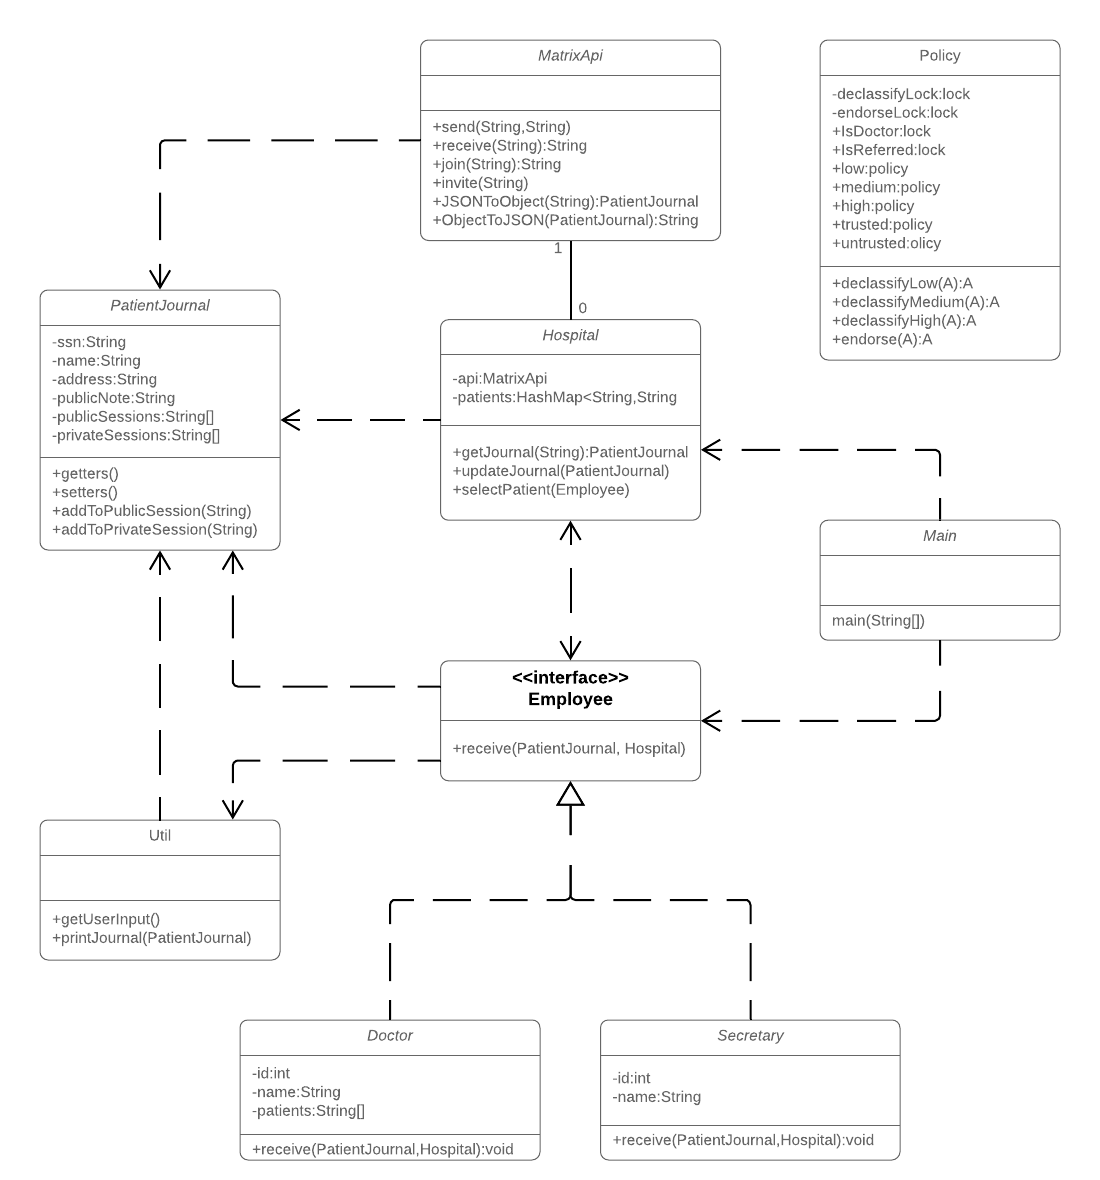
\includegraphics[width=12cm]{figures/journalsystem_class.png}
	\caption{Class diagram for the Journal system}
	\label{fig:journalsystem}
\end{figure}



\subsubsection{Matrix}


%Matrix API's




Configurations for room:
- Rooms are precreated and each hospital are aware of each room. 
- Hospitals in a Room are preconfigured and every client knows from the beginning which hospitals are in the room / or can join the room.
- The room is invite-only
- Default user level is 100. Anyone can kick, ban and invite users. 


\begin{figure}[H] 
	\hspace*{-1cm}
	\centering
	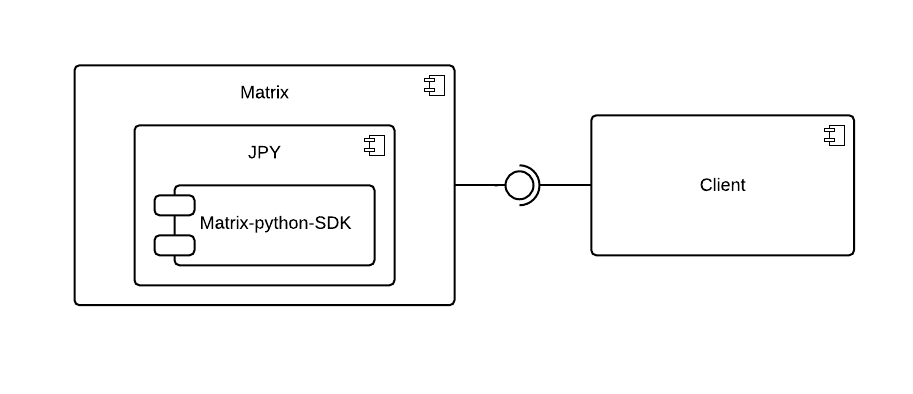
\includegraphics[width=14cm]{figures/matrix_component.png}
	\caption{Matrix interface}
	\label{fig:matrix_component}
\end{figure}



\subsubsection{Limitations}

%Incompatibility with Paragon

A design problem is the concurrent writes to a journal from multiple hospital. Before writing to a journal; the latest version of the journal in Matrix is first retrieved and then the writes are appended to the journal. However multiple hospitals might have retrieved the latest journal and different doctors might have committed changes to the journal and send it to Matrix hence one of the writes would be lost since only the latest journal is retrieved.

This is a common issue in distributed systems but is not handled in this solution. 


% It is assumed that a version control mechanism is in place and the latest journal received is always up to date.
% Solution merging data like version control systems like git.



\section{Paragon implementation}

\subsection{The Matrix interface}


\subsection{Policies and locks}

%D Declaration examples

\subsubsection{Lattice}

\subsection{Declassification}

\subsection{Exception handling}


\subsection{Limitations}

The Matix 
Technical requirements:
-Msg type should be "m.text" when sending patient journal (JSON format). The convertion of string to JSON and vice versa should happen in the client.

\section{Summary}